Zwei der vorgestellten Spielideen werden mit Hilfe der ben�tigten Features als Android-App implementiert. Hierzu wird ein Framework entwickelt, das allgemein ben�tigte Funktionalit�ten bereitstellt, und darauf aufbauend werden die beiden Beispielspiele umgesetzt.

<<<<<<< HEAD

\section{Allgemeines Framework}
%\subsection{Spiellogik}
Unser System besteht aus zwei Komponenten. Eine Android-App mit der gesamten Spiellogik und einem Server �ber den die Kommunikation zwischen den mobilen Endger�ten abl�uft.

\subsection*{Server}
Der implementierte Server arbeitet mit Java und ZeroMQ. Er �ffnet zwei Kommunikationskan�le mit dem Client. Der erste ist ein ZeroMQ-Request-Reply-Socket-Paar, �ber das die Endger�te Nachrichten an den Server senden. Der zweite ist ein Publish-Subscribe-Socket-Paar, �ber das die Nachrichten an Gruppen von Endger�ten weitergeleitet werden. Eine Nachricht besteht aus drei Teilen: einer Adresse, dem Nachrichtentyp und einem serialisierten Objekt vom Typ TransferObject (siehe Abbildung \ref{fig:transfer}). Die Adresse ist entweder die ID eines Spielers oder die ID einer Spielinstanz. Wir nutzen ZeroMQs Multipart-Message-Feature um diese Teile voneinander getrennt bei der Kommunikation zu �bermitteln. Der Server sendet eingehende Nachrichten an bestimmte Clients weiter. Das kann entweder ein einzelner Client, oder alle Clients die sich in einer Spielsession befinden, sein. Der Server kennt dabei den Zustand der einzelnen Spiele nicht. Um mehrere Spielinstanzen gleichzeitig verwalten zu k�nnen, h�lt er aber eine Liste aller laufenden Spiele samt Informationen dar�ber, welcher Spieler an welchem Spiel teilnimmt. Wenn eine Nachricht vom Typ "`create\_game"' empfangen wird tr�gt der Server die ID des Spiels in eine Liste ein. Diese Liste wird einem Client gesendet wenn er sie �ber eine entsprechende Nachricht anfragt.
=======
\section{Allgemein}
\section{GUI}

Die GUI (Grafic User Interface) wurde nur mit den Android bzw. GooglePlay Services (inkl. Googlemaps) um gesetzt. Die mitgelieferten
M�glichkeiten des Android SDK sind in dieser Hinsicht f�r die GUI-Umsetzung dieses Projektes vollkommen zufriedenstellend. Die komplette
GUI setzt sich aus 2 Activities zu sammen, die im folgenden ein wenig genauer beleuchtet werden.

\subsection*{Login-Screen}
Diese Activity wird zuerst aufgerufen und zeigt einen Bildschirm auf dem sich der Spieler einen Benutzernamen aussucht und danach mit dem
"`Start"' Button zu n�chsten Activity wechselt, welche das eigentliche Spiel zeigt.

\begin{wrapfigure}{r}{0.5\textwidth}
  \begin{center}
    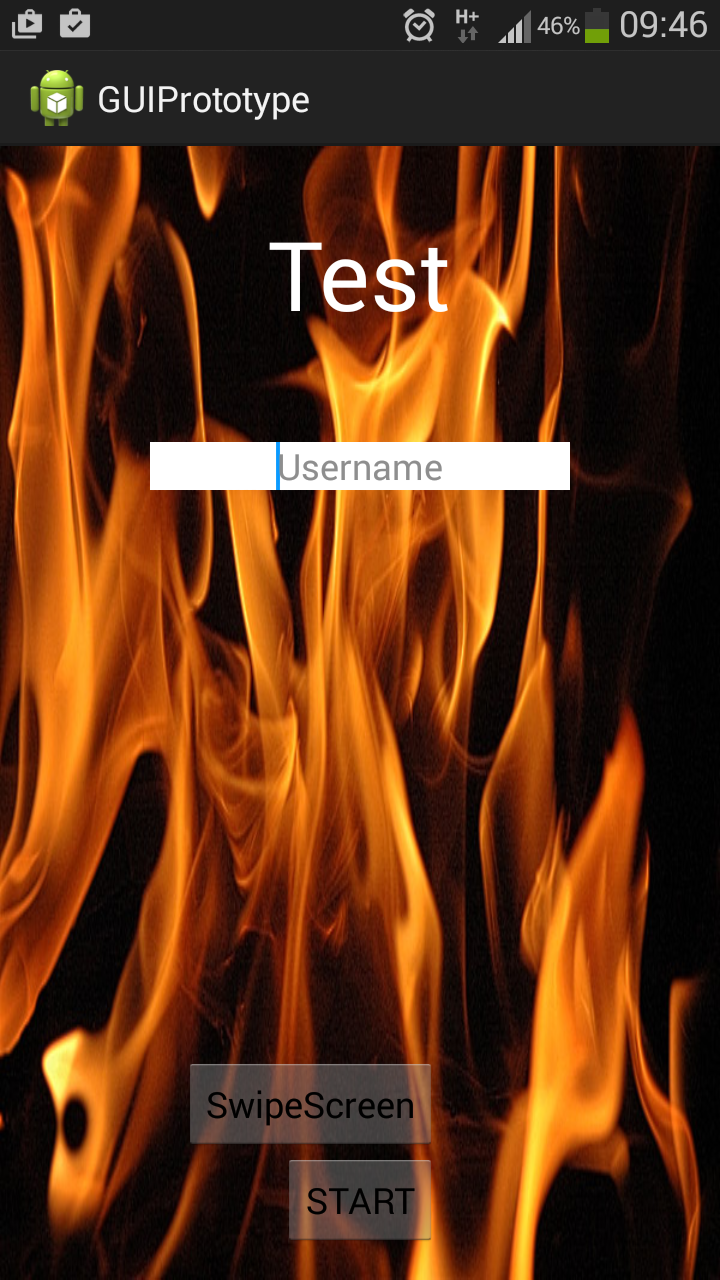
\includegraphics[width=0.48\textwidth]{4-Technische_Loesungen/4-5-GUI/Data/login_screen.png}
     \caption{Login Screen}
  \end{center}
\end{wrapfigure}


\subsection*{Swipe-Screen}
Schon in der sehr fr�hen Entwicklungsphase war festzustellen, das die verschiedenen Elemente der GUI - wie im folgenden weiter erl�utert- zu zahlreich sind, um sie auf einen Bildschirm umzusetzen. Die eigentliche Kartendarstellung w�re sonst zu klein gewesen. Also wurde entschieden die verschiedenen Elemente auf weitere Bildschirme zu verteilen. In den ersten entw�rfen geschah dies �ber einzelne Activities, also mehrere Bildschirme. Um gewisse Android Komfort-Funktionen und Gesten dem Nutzer zu verf�gung zu stellen wurden die zun�chst eigenst�ndigen Activites zu Fragments umgebeut, die dann in einem so genannten Swipe-Screen zusammengefasst werden. In diesem werden die Fragments als Tabs organisiert und der User kann entweder durch "`wischen"' (swipe) oder durch klicken auf die Tabs durch die GUI Navigieren. \newline
Ein weiterer Vorteil ist ebenfalls, dass benachbarte Tabs jeweils ein wenig {\color{red}'ein wenig' streichen} vorgeladen (Laden der Widgets) bzw. noch im Speicher behalten werden. Zum einen wird so sichergestellt, dass der Tab-Wechsel per wischen "`geschmeidig"' abl�uft, aber auch gibt es so nur sehr geringe Ladezeiten zwischen den einzelenen Bildschirmen. Zudem ist die von Google angepriesene "`Wiederverwendbarkeit"' von Fragments als UI (User Interface) ebenfalls n�tzlich, wenn weitere �hnliche Spiele umgesetzt werden sollen.

\begin{wrapfigure}{r}{0.5\textwidth}
  \begin{center}
    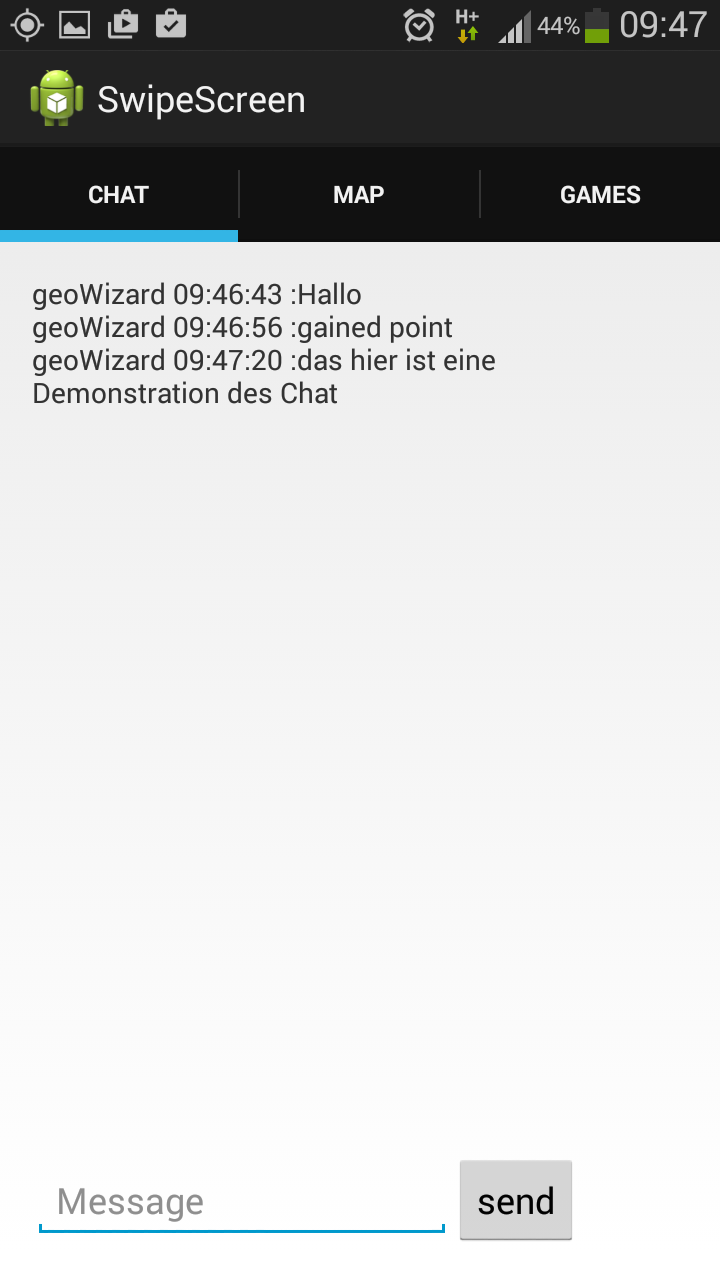
\includegraphics[width=0.48\textwidth]{4-Technische_Loesungen/4-5-GUI/Data/chat_screen.png}
     \caption{Chat Screen}
  \end{center}
\end{wrapfigure}

\subsubsection*{Chat-Screen}
In desem Fragment wird die m�glichkeit des Chattens zwischen mehreren Spielern umgesetzt. Die grafische Umsetzung des Chats wurde der von IRC (Instant Relay Chat) Clients nachempfunden und ist entsprechend simpel gel�st. Es wird der jeweilige Benutzername, Uhrzeit und die eigentliche Nachricht angezeigt. Die Eingabe der Chat-Nachricht erfolgt in einem Text-Eingabe-Feld. Die Anzeige der Chat-Nachrichten erfolgt in einem einfachen Textanzeige-Feld (TextView\footnote{{\color{red}\url{Link zur Android-Doku}}}) was wiederum in einem scrollbaren Feld (SrcollView\footnote{{\color{red}\url{Link zur Android-Doku}}}) liegt. Hierdurch ist es m�glich durch alle empfangenen Nachrichten "`durchzuscrollen"'. Wird eine Chat-Message (genaueres in Kapitel 4.4) empfangen, wird diese mittels Stringmanipulation an das Textfeld angeh�ngt. Hierbei ist zu beachten, dass die selbst verschickten Nachrichten erst an den Server gesendet werden und dann jeweils an die entsprechenden Nutzer. Somit kann es aufgrunde von �bertragungsverz�gerungen dazu kommen, das die eigene Nachricht verz�gert angezeigt, jedoch ist die korrekte Reihenfolge der Nachrichten gewahrt.

\newpage

\begin{wrapfigure}{r}{0.5\textwidth}
  \begin{center}
    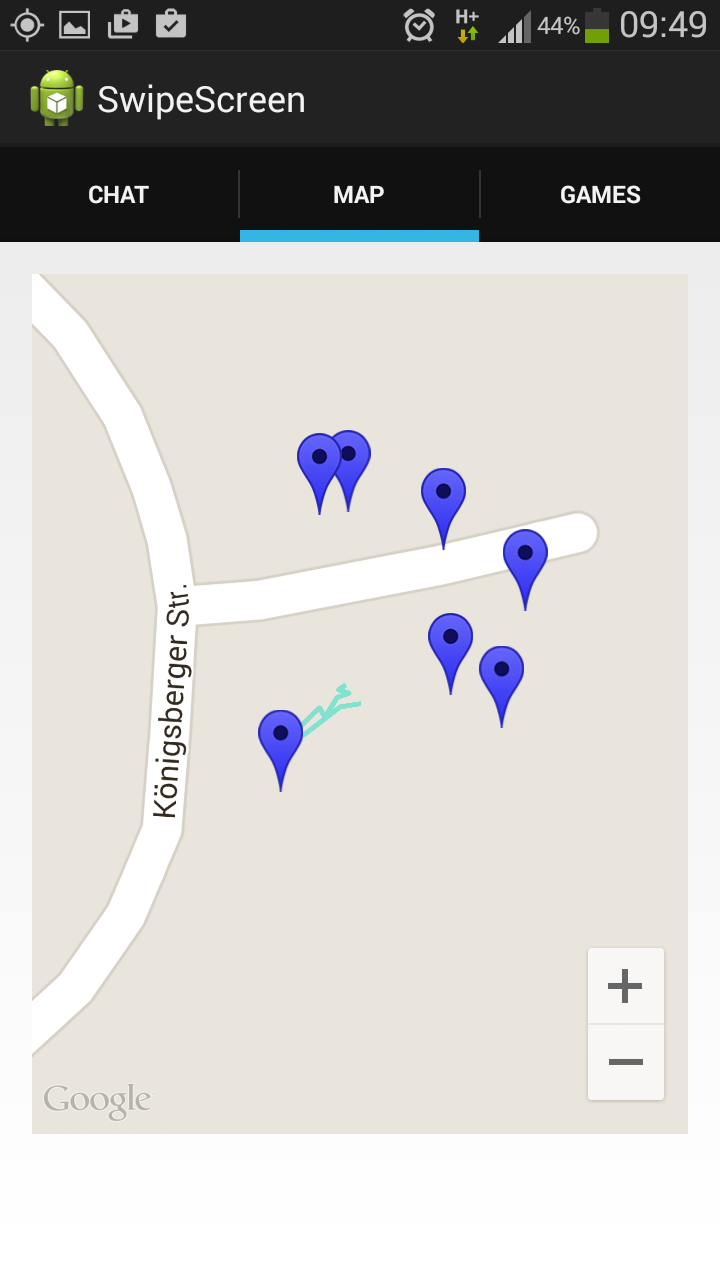
\includegraphics[width=0.48\textwidth]{4-Technische_Loesungen/4-5-GUI/Data/map_screen.png}
     \caption{Map Screen}
  \end{center}
\end{wrapfigure}

\subsubsection*{Map-Screen}
In diesem Fragment wird die Karte in einem weiterem Fragment angezeigt. Je nachdem welches Spiel gespielt wird zu zus�tzliche Widgets vorhanden, wie z.B. Interaktions Buttons, (Team-)Punkte anzeige usw.


\subsubsection*{Game-Screen}
In diesem Fragment werden momentan aktive Spiele angezeigt. Auch ist es m�glich neue Spiele zu erstellen. Die Anzeige der Liste der Spiele erfolgt in einer scrollf�higen Liste (ListView). Diese wird durch entsprechend angefordete Informationen �ber andere Spiele geupdatet. Diese Informationen werden durch Anfrage bei anderen Benutzer die sich eingeloggt haben �ber einen bestimmen Message-Typ abgerufen. Die Listen-Elemente sind interaktiv. Ein klick auf das entsprechende Spiel startet den beitritt. Um ein Spiel eines gewissen Typs zu Starten w�hlt man in einen Dropdown-Men� (bei Android Spinner) den entsprechenden Modus aus in klickt auf create. Man selbst betritt dieses Spiel und eintrag in der Spiele-Liste wird vorgenommen. 


\begin{figure}[r]  
    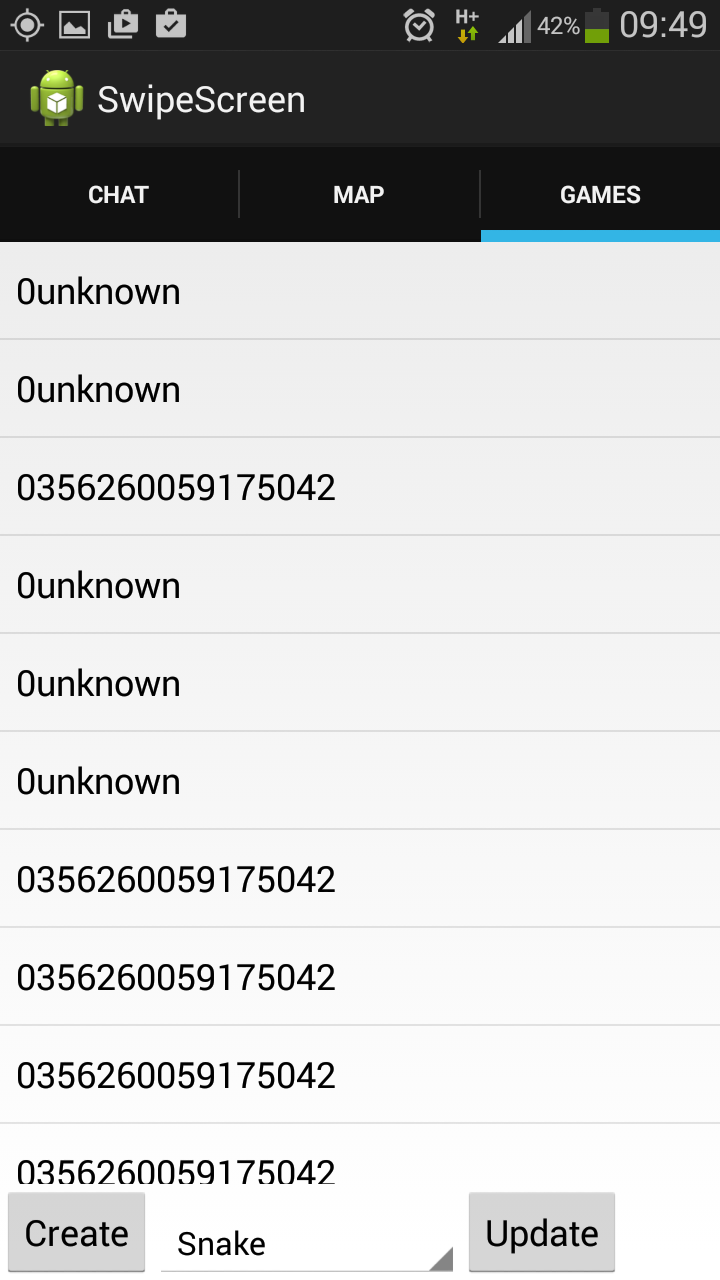
\includegraphics[width=0.48\textwidth]{4-Technische_Loesungen/4-5-GUI/Data/game_screen.png}
    \caption{Game Screen}
\end{figure}

\clearpage

\subsection{Spiellogik}
Unser System besteht aus zwei Komponenten. Eine Android-App mit der gesamten Spiellogik und einem Server �ber den die Kommunikation zwischen den mobilen Endger�ten abl�uft.

\subsubsection{Server}
Der implementierte Server arbeitet mit Java und ZeroMQ. Er �ffnet zwei Kommunikationskan�le mit dem Client. Der erste ist ein ZeroMQ-Request-Reply-Socket-Paar, �ber das die Endger�te Nachrichten an den Server senden. Der zweite ist ein Publish-Subscribe-Socket-Paar, �ber das die Nachrichten an Gruppen von Endger�ten weitergeleitet werden. Eine Nachricht besteht aus drei Teilen: einer Adresse, dem Nachrichtentyp und einem serialisierten Objekt vom Typ TransferObject (siehe Abbildung \ref{fig:transfer}). Die Adresse ist entweder die ID eines Spielers oder die ID einer Spielinstanz. Wir nutzen ZeroMQs Multipart-Message-Feature um diese Teile voneinander getrennt bei der Kommunikation zu �bermitteln. Der Server sendet eingehende Nachrichten an bestimmte Clients weiter. Das kann entweder ein einzelner Client, oder alle Clients die sich in einer Spielsession befinden, sein. Der Server kennt dabei den Zustand der einzelnen Spiele nicht. Auf dem Server befindet sich eine Liste von momentan aktiven Spielen. Wenn eine Nachricht vom Typ "`create\_game"' empfangen wird tr�gt der Server die ID des Spiels in eine Liste ein. Diese Liste wird einem Client gesendet wenn er sie �ber eine entsprechende Nachricht anfragt. Dabei werden vorher Spiele aus der Liste gel�scht, bei denen in den letzten 5 Minuten keine Nachricht auf dem Server empfangen wurde.
>>>>>>> origin/master




%
%\begin{figure}
%	\begin{center}
%		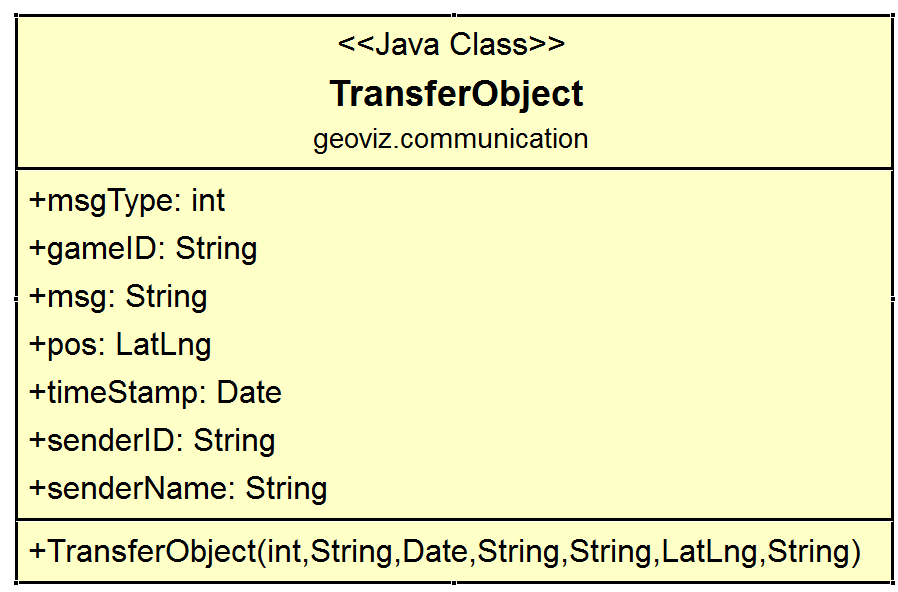
\includegraphics[width=0.5\textwidth]{img/transferobject.png}
%		
%		\caption{UML-Diagramm der Klasse\newline geoviz.communication.TransferObject}
%		\label{fig:transfer}
%	\end{center}
%\end{figure}

<<<<<<< HEAD
\subsection*{Client}
Unsere Android-Applikation besteht aus drei Fragmenten zwischen denen man durch Wischen wechseln kann. Das erste Fragment ist ein Chat �ber den Spieler Textnachrichten an ihre Mitspieler im gleichen Spiel senden k�nnen.
=======
\subsubsection{Client}
%Unsere Android-Applikation besteht aus drei Fragmenten zwischen denen man durch Wischen wechseln kann. Das erste Fragment ist ein Chat �ber den Spieler Textnachrichten an ihre Mitspieler im gleichen Spiel senden k�nnen.
>>>>>>> origin/master

Im Hintergrund laufen zwei Threads f�r die Kommunikation. Der eine k�mmert sich um den Empfang von Nachrichten und beinhaltet einen ZeroMQ-Subscriber-Socket. Dieser empf�ngt alle Nachrichten, die vom Publisher"=Socket auf dem Server direkt an die ID des Clients oder die ID des Spiels, in dem er sich befindet, adressiert sind. Der zweite Thread sendet Nachrichten an den Server. 
Bei einem Spielbeitritt einer laufenden Session, wird �ber den Server eine Anfrage des aktuellen Status des Spiels an alle momentanen Mitspieler gesendet, welche den Zustand des Spiels alle an den anfragenden Client zur�cksenden. Dieser beachtet nur die erste Nachricht und verwirft den Rest.
Des weiteren l�uft ein LocationClient, welcher immer die aktuelle Position als Nachricht an alle Spieler der selben Spielinstanz weiterschickt. 


%Das zweite Fragment ist die Karte auf der wir unser Spiel darstellen.  
%F�r die Darstellung der Karte verwenden wir GoogleMaps. 

%Im dritten Fragment kann ein Spieler eine neue Spielinstanz erstellen oder einem bereits laufendem Spiel beitreten. Die Liste der momentan laufenden Spiele wird per Knopfdruck vom Server abgefragt. Wenn man einer laufenden Session beitritt wird �ber den Server eine Anfrage des aktuellen Status des Spiels an alle momentanen Mitspieler gesendet, welche den Zustand des Spiels alle an den anfragenden Client zur�ck senden. Dieser beachtet nur die erste Nachricht und verwirft den Rest.



 


